\subsection{Obsługa programu}
Program do uruchomienia wymaga zainstalowanego Pythona w wersji 3.11

Przed uruchomieniem programu należy zainstalować wymagane paczki z pliku \verb|requirements.txt| znajdującego się w folderze \verb|Code|.

Następnie program można uruchomić używając polecenia \verb|python main.py| w folderze \verb|Code|.

Po uruchomieniu programu zostaną automatycznie wczytane ustawienia z pliku \verb|app_settings.json|. Jeśli plik ten nie zostanie znaleziony, zostanie on automatycznie utworzony z użyciem podstawowych ustawień programu. Następnie wyświetli się następujący ekran

\begin{figure}[H]
	\centering
		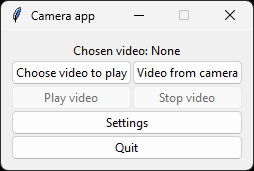
\includegraphics[width=0.5\textwidth]{Img/manual/main_screen.png}
	\caption{Ekran główny programu}
	\label{fig:main_screen}
\end{figure}

W celu wybrania pliku mp4 do odtworzenia w programie, należy nacisnąć przycisk \verb|Choose video to play|. Otworzy się wtedy systemowy eksplorator plików w którym należy wybrać plik wideo, który chcemy załadować do programu.

Po poprawnym załadowaniu pliku video, napis \verb|None| przy \verb|Chosen| video zostanie zastąpiony jego nazwą.

\begin{figure}[H]
	\centering
	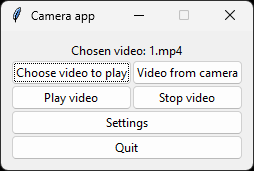
\includegraphics[width=0.5\textwidth]{Img/manual/video_loaded.png}
	\caption{Program po załadowaniu nagrania}
	\label{fig:video_loaded}
\end{figure}

Alternatywnie, naciśnięcie przycisku \verb|Video from camera| połączy program z kamerą podłączoną do komputera. W miejscu \verb|None| pojawi się wyraz \verb|Camera|.

\begin{figure}[H]
	\centering
	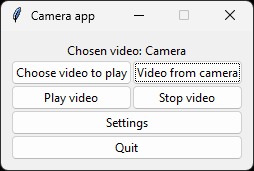
\includegraphics[width=0.5\textwidth]{Img/manual/camera_loaded.png}
	\caption{Program po wybraniu kamery}
	\label{fig:camera_loaded}
\end{figure}

Po wybraniu jednej z powyższych opcji, odblokowane zostaną przyciski \verb|Play video| oraz \verb|Stop video|.

\newpage

Naciśnięcie przycisku \verb|Play video| spowoduje uruchomienie wybranego nagrania, lub otworzenie podglądu kamery na żywo.

Przycisk \verb|Stop video|o zatrzyma odtwarzanie i zamknie okno z nagraniem lub podglądem kamery.

\begin{figure}[H]
	\centering
	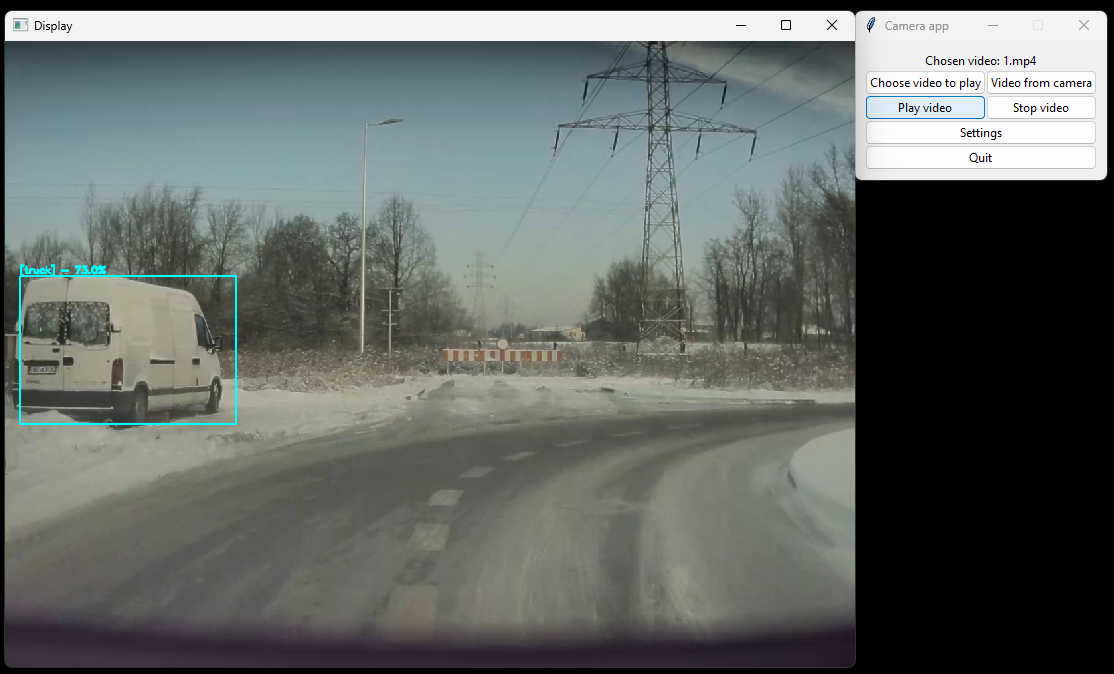
\includegraphics[width=0.9\textwidth]{Img/manual/video_playing.png}
	\caption{Program po uruchomieniu nagrania}
	\label{fig:video_playing}
\end{figure}

Rozmiar okna z nagraniem może być zmieniany a jego pozycja śledzi pozycje głównego okna programu.

\newpage

Naciśnięcie przycisku \verb|Settings| spowoduje otworzenie okna ustawień, które jest połączone z głównym oknem programu.

\begin{figure}[H]
	\centering
	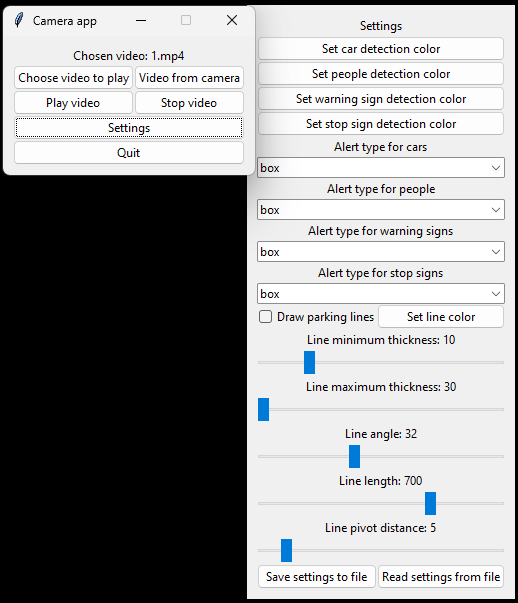
\includegraphics[width=0.9\textwidth]{Img/manual/settings_opened.png}
	\caption{Program z otwartym menu ustawień}
	\label{fig:settings_opened}
\end{figure}

\newpage

Pierwsze cztery przyciski \verb|Set … detection color| pozwalają na edytowanie kolorów obramówek wykrywanych obiektów.
Idąc od góry są to odpowiednio: 1. samochody, 2. piesi, 3. znaki ostrzegawcze, 4. znaki stopu.

\begin{figure}[H]
	\centering
	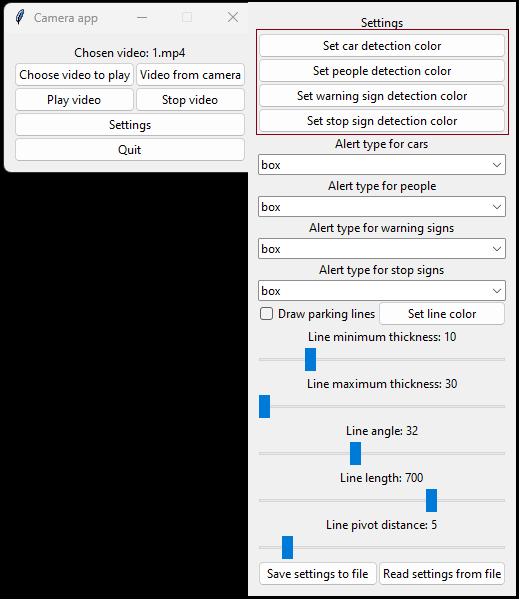
\includegraphics[width=0.9\textwidth]{Img/manual/color_settings.png}
	\caption{Ustawienia kolorów}
	\label{fig:color_settings}
\end{figure}

\newpage

Zaznaczając pole \verb|Draw parking lines| możemy włączyć lub wyłączyć nakładanie linii pomocniczych na wyświetlany obraz.

Przycisk \verb|Set line color| pozwala zmienić kolor linii pomocniczych.

Suwaki znajdujące się poniżej pozwalają zmieniać parametry linii pomocniczych.
Idąc od góry są to: 1. minimalna grubość linii, 2. maksymalna grubość linii, 3. Kąt nachylenia linii, 4. długość linii, 5. odległość punktu zaczepienia linii.

\begin{figure}[H]
	\centering
	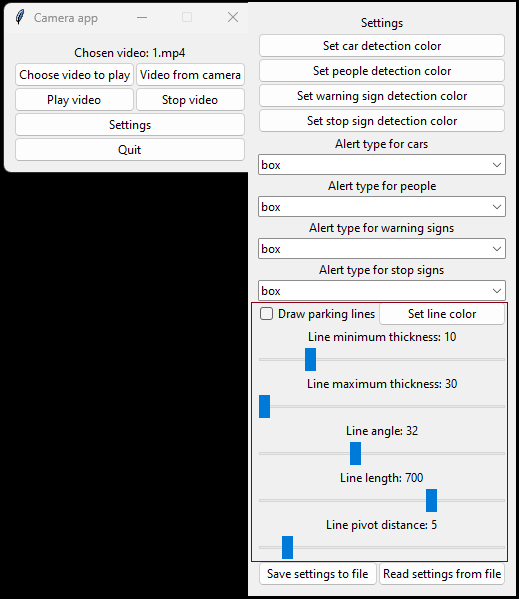
\includegraphics[width=0.9\textwidth]{Img/manual/line_settings.png}
	\caption{Ustawienia linii pomocniczych}
	\label{fig:line_settings}
\end{figure}

\newpage


Przycisk \verb|Save settings to file| zapisuje aktualne ustawienia do pliku. Jeśli ustawienia nie zostaną zapisane, to zostaną one utracone po wyjściu z programu.

Przycisk  \verb|Read settings from file| pozwala wczytać ustawienia z pliku zewnętrznego, jeśli został on zmieniony zewnętrznie w trakcie działania programu.

Po naciśnięciu dowolnego z tych przycisków, wyświetlone zostanie okienko potwierdzające poprawne wykonanie akcji.


\begin{figure}[H]
	\centering
	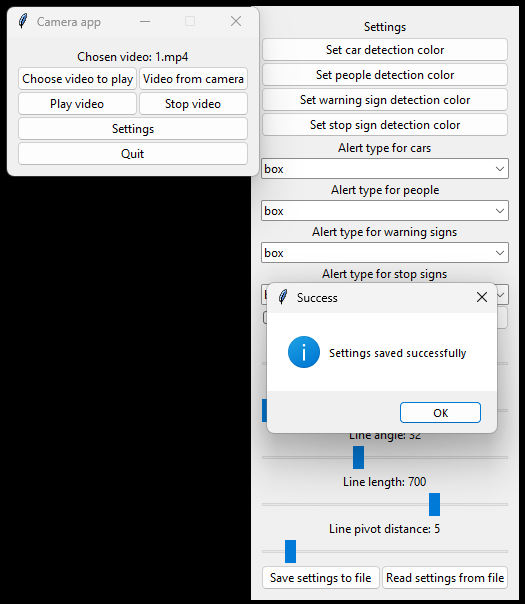
\includegraphics[width=0.9\textwidth]{Img/manual/settings_saved.png}
	\caption{Poprawne zapisanie ustawień}
	\label{fig:settings_saved}
\end{figure}

Naciśnięcie przycisku \verb|Quit| spowoduje wyjście z programu.

\subsection{Interpretacja zachowania programu}

W trakcie odtwarzania pliku wideo lub analizy obrazu z kamery, program będzie wykrywał określone rodzaje obiektów i ostrzegał przed nimi w wybrany przez użytkownika sposób.

Obiekty, dla których wybrana została opcja box będą otaczane obramówką w wybranym przez użytkownika kolorze.

W przypadku opcji alertu dźwiękowego, program będzie odtwarzał dźwięk ostrzegawczy gdy na obrazie wykryty jest przynajmniej jeden obiekt dla którego wybrany został alert dźwiękowy.




